\chapter{Basics}

\section{JavaScript}
There are a few big advantages offered by \textbf{\gls{JS}. Maybe the biggest advantage is that it comes with the web browser, so everybody can run it by simply typing in an \gls{URL}}. This offers great possibilities, since the users don't have to install any software package. The provided application is immediately ready to use once it was loaded. Today \gls{JS} is the most used programming language world wide. 
\gls{JS} first appeared in 1995, originally developed at Netscape by Brendan Eich it had a simple purpose, dynamically manipulating the HTML DOM in the browser. At the same time a company called Sun worked on a programming language called Java, Netscape and Sun decided to work together. Netscape noticed that it would be good marketing to rename LiveScript to \gls{JS}. Since Java already had a growing community and was liked by many people, so Netscape took the chance and \gls{JS} was born. However both language don't share a lot of things together, Java is a normal, static, and highly typed programming language, it runs on a virtual machine and needs to be compiled, whereas the single threaded \gls{JS} only runs in the browser and is script. Nevertheless they share the C related syntax and some similarities regarding naming conventions, both support object oriented programming. Jeff Attwood the co-founder of the  computer programming question-and-answer website Stack Overflow and Stack Exchange once said "Any application that can be written in \gls{JS}, will eventually be written in JavaScript".

\begin{figure}[hb]
	\centering
	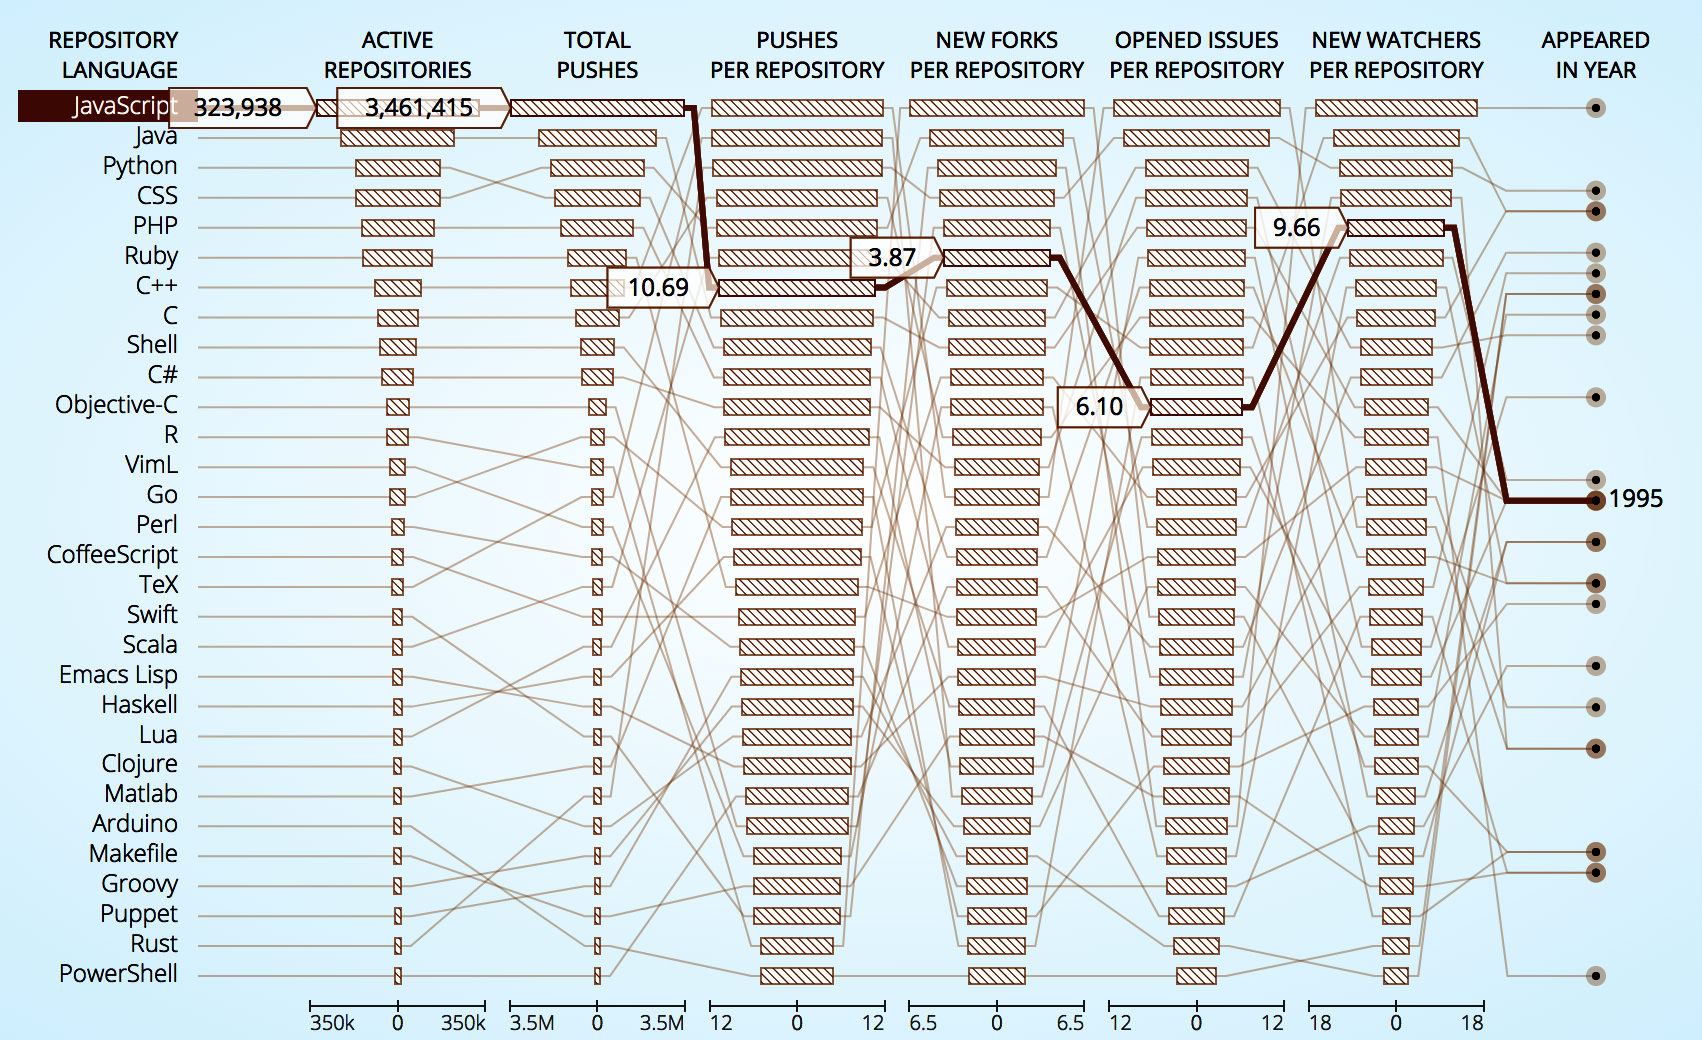
\includegraphics[scale=0.5]{bilder/grundlagen/jsUsage.png}
	\caption{Github Repositories sorted after used language} Source:\cite{JSUSAGE}
	\label{fig:JSUSAGE}
\end{figure}


\subsection{Software}
Zur Programmierung der Software wird MATLAB\textregistered\ (2017b) mit Simulink\textregistered\ und dessen Emebedded Coder\texttrademark\ ,\ sowie die Image Processing Toolbox\texttrademark\ verwendet.


\begin{figure}[hb]
	\centering
	
\includegraphics[scale=0.5]{bilder/MATLABLogo.png}
	\caption{MATLAB Logo}
	\label{fig:MATLAB}
\end{figure}



